% MCTA-Bench --- draft for the NeurIPS 2026 FAST workshop.
%
% Compiles as-is on Overleaf with pdfLaTeX: no .bib run, no external images, no
% style file to download. The bibliography is inline and the figures are TikZ.
%
% To switch to the workshop template, download neurips_2026.sty, then replace the
% \documentclass line and the geometry package with:
%     \documentclass{article}
%     \usepackage[final]{neurips_2026}     % or \usepackage{neurips_2026} while anonymous
% and delete the \geometry{...} line below. Everything else carries over.

\documentclass[10pt]{article}

\usepackage[utf8]{inputenc}
\usepackage[T1]{fontenc}
\usepackage[margin=1in]{geometry}
\usepackage{amsmath,amssymb}
\usepackage{booktabs}
\usepackage{microtype}
\usepackage{graphicx}
\usepackage{float}
\usepackage{tikz}
\usetikzlibrary{arrows.meta,positioning}
\usepackage[hidelinks]{hyperref}
\usepackage{url}

% Default float parameters leave large gaps when several tables compete for the
% top of a page; these let floats share a page with more text.
\renewcommand{\topfraction}{0.9}
\renewcommand{\bottomfraction}{0.8}
\renewcommand{\textfraction}{0.07}
\renewcommand{\floatpagefraction}{0.75}
\setcounter{topnumber}{3}
\setcounter{totalnumber}{4}

\newcommand{\MCTA}{\textsc{Minimum-Cost Task Alignment}}
\newcommand{\tw}{\mathrm{tw}}

\title{Nudging the Graph, Not the Agent:\\
       A Benchmark for Alignment by Environment Design}

% Anonymised for double-blind review; restore for the camera-ready.
\author{Anonymous Authors}
\date{}

\begin{document}
\maketitle

\begin{abstract}
Agent harnesses are environments: the tools on offer, the ordering of steps and
the presence of shortcuts determine not only what an agent \emph{can} do but what
it \emph{will} do. Practitioners already align agents by editing these
environments---removing a tool, forcing a checkpoint, blocking a shortcut---without
a formal objective, a solver, or any guarantee that an edit constrains
\emph{every} trajectory the agent might sample. The Kleinberg--Oren model of
present-biased planning on task graphs formalises exactly this setting, and the
accompanying \MCTA{} problem asks for the cheapest edit forcing every feasible
trajectory to reach the goal and perform a prescribed set of critical actions. The
theory is well developed and has never been executed. We release MCTA-Bench: 18\,045
task graphs from four domains---agent tool decompositions, university curricula and
scientific workflow traces---
annotated with the structural parameters that govern tractability; six parametric
instance families whose decision thresholds are placed analytically; exact and
heuristic solvers; and an agent-in-the-loop probe that recovers an agent's discount
factor exactly rather than by fitting. Real task graphs turn out structurally
narrow---treewidth in single digits where prior measurements of network data report
hundreds---yet two of seven workflow families remain intractable regardless,
because tractability turns on weight diversity as much as on width. The repair an
engineer would make by hand matches the optimum on the median real instance and
costs up to $2.67\times$ more in the tail, on instances of treewidth two. On
general graphs no language-model agent we tested shows present bias, at any
capability. But the benchmark's inspection tooling led us to a structural
configuration where one model does, reliably and repeatedly---a large step toward
the goal beside cheap ways of postponing it---and another does not at all. The
behavioural premise therefore holds in an identifiable class of environments rather
than universally, while the intervention machinery transfers intact: theory-derived
edits move compliance from $0\%$ to $100\%$ across the whole sampling distribution,
computed for a discount factor the agent does not have.
\end{abstract}

\section{Introduction}

Designing an agent's harness is already alignment work. Which tools are exposed,
which steps are mandatory, whether a cheap shortcut sits beside the thorough
route---these choices shape behaviour more reliably than instructions do, and
practitioners make them constantly. They make them by intuition. There is no
objective being minimised, no solver, and no way to check that an edit binds every
trajectory the agent might produce rather than the one it happened to produce
during testing.

A formal account exists. Kleinberg and Oren~\cite{kleinberg2014} model an agent
traversing a task DAG that evaluates plans under a present-biased discount: the
next action counts in full, everything after it is discounted by $\beta$. Such an
agent can announce a sensible plan and abandon it on arrival, with nothing about
the environment having changed in between. The principal cannot alter $\beta$ but
can edit the graph, and \MCTA{}~\cite{belova2024,belova2026} asks for the cheapest
edit forcing every feasible trajectory to reach the target and traverse a
prescribed set of critical arcs.

This line has produced a detailed complexity landscape and no experiments. Nobody
has run the algorithms, measured the environments they assume, or checked the
behavioural premise against an actual agent. Each needs a benchmark that does not
exist: instances real enough to say something about deployment, annotated with the
parameters the theory is stated in, and solvers trustworthy enough to compare
against.

One observation frames the exercise. An agent sampling at temperature above zero is
precisely the nondeterministic tie-breaker the model's all-feasible-paths
formulation is written for. Prompting shifts the \emph{mode} of an agent's
behaviour; editing its environment is supposed to constrain the entire
\emph{support}. That distinction is what a theory of environment design buys over
instruction-writing, and it is testable.

\section{Setting}

An instance is $M = (G, w, s, t, \beta, r)$ with $G$ a weighted DAG. Standing at
$v$, the agent evaluates every $v$--$t$ path under
\[
  \zeta(P) \;=\; w(e_1) + \beta \sum_{i \geq 2} w(e_i),
\]
abandons if $\min_P \zeta(P) > \beta r$, and otherwise commits to $e_1$ and
repeats. Ties are broken arbitrarily, so the model induces a \emph{set} of feasible
trajectories rather than a single path. \MCTA{} seeks $S \subseteq E$ minimising
$\sum_{e \in S} c(e)$ such that in $G - S$ every feasible trajectory reaches $t$ and
traverses every arc of $T$. Costs are real-valued, so an auxiliary arc with a
negative deletion cost is one the solver pays to \emph{keep}: a single objective
carries both deletion and paid addition. Figure~\ref{fig:example} shows why blocking
the tempting route is not generally enough.

\begin{figure}[t]
\centering
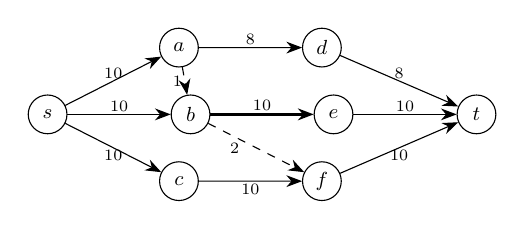
\begin{tikzpicture}[
  scale=0.82, transform shape,
  >={Stealth[length=2mm]},
  every node/.style={font=\small},
  st/.style={circle,draw,minimum size=6mm,inner sep=0pt},
  w/.style={font=\scriptsize,inner sep=1pt}
]
\node[st] (s) {$s$};
\node[st,above right=6mm and 16mm of s] (a) {$a$};
\node[st,right=16mm of s]              (b) {$b$};
\node[st,below right=6mm and 16mm of s] (c) {$c$};
\node[st,right=16mm of a] (d) {$d$};
\node[st,right=16mm of b] (e) {$e$};
\node[st,right=16mm of c] (f) {$f$};
\node[st,right=16mm of e] (t) {$t$};

\draw[->] (s) -- node[w,above]{10} (a);
\draw[->] (s) -- node[w,above]{10} (b);
\draw[->] (s) -- node[w,below]{10} (c);
\draw[->] (a) -- node[w,above]{8}  (d);
\draw[->] (c) -- node[w,below]{10} (f);
\draw[->] (d) -- node[w,above]{8}  (t);
\draw[->] (f) -- node[w,below]{10} (t);
\draw[->] (e) -- node[w,above]{10} (t);

\draw[->,very thick] (b) -- node[w,above]{10} (e);
\draw[->,dashed] (b) -- node[w,pos=0.35,below left]{2} (f);
\draw[->,dashed] (a) -- node[w,left]{1} (b);
\end{tikzpicture}
\caption{The worked example, after~\cite{belova2026}. With $\beta = 1/2$ and
$r = 36$ the agent walks $sbft$, skipping the critical arc $(b,e)$ (thick).
Deleting the shortcut $(b,f)$ only diverts it to $sadt$, which also skips $(b,e)$;
adding the auxiliary arc $(a,b)$ yields $sabet$. Our simulator reproduces every
perceived cost the paper states, and those numbers are the test suite.}
\label{fig:example}
\end{figure}

\section{MCTA-Bench}
\label{sec:bench}

The benchmark has three parts: instances derived from published data, instance
families generated to a specification, and the tooling that makes both measurable.

\subsection{A taxonomy of instances}

\begin{table}[t]
\centering
\small
\begin{tabular}{llrrrrr}
\toprule
Domain of origin & Source & Instances & Branching & Discrim. & Arcs (med.) & $\tw$ \\
\midrule
\multicolumn{7}{l}{\emph{Agent task decompositions} --- synthetic weights} \\
\quad everyday APIs   & TaskBench~\cite{taskbench} & 4\,318 &   275 &   0 & 2--9 (4)     & 2 \\
\quad multimedia      & TaskBench                  & 5\,548 &   525 &  21 & 2--11 (4)    & 2 \\
\quad HuggingFace     & TaskBench                  & 7\,435 &   775 &  42 & 2--11 (4)    & 2 \\
\midrule
\multicolumn{7}{l}{\emph{Human curricula} --- synthetic weights} \\
\quad Caltech         & \cite{stavrinides2023}     &   169 &   169 &  28 & 7--30 (14)   & 4 \\
\quad Johns Hopkins   & \emph{ibid.}, from prose   &   533 &   495 & 119 & 6--180 (23)  & 6 \\
\midrule
\multicolumn{7}{l}{\emph{Scientific workflows} --- \textbf{measured runtimes}} \\
\quad montage         & WfCommons~\cite{wfcommons} &     6 &     6 &   5 & 130--1336 (365) & 18 \\
\quad soykb           & WfCommons                  &     6 &     6 &   2 & 202--757 (479)  & 12 \\
\quad five others     & WfCommons                  &    30 &    30 &   1 & 42--1201        & 2--3 \\
\bottomrule
\end{tabular}
\caption{What each domain of origin supplies. \emph{Branching} counts instances
with any node offering a choice of continuation; fan-in---several inputs to one
task---is not a decision. \emph{Discriminating} counts those on which a patient and
a biased agent walk different routes, which is the only kind that can measure an
agent at all. Reproduce with \texttt{scripts/taxonomy.py}.}
\label{tab:corpus}
\end{table}

Table~\ref{tab:corpus} is the benchmark's central artefact, and its middle columns
carry a result. \textbf{The domain agents actually operate in barely produces
environments that can pose the question.} Of 17\,301 agent task decompositions,
1\,575 contain any choice of continuation and 63 are discriminating; the everyday
API domain contains none whatsoever. Their dependency structure is overwhelmingly
fan-in, and their graphs are tiny---a median of four arcs, treewidth two. Human
curricula, designed by people for people, are markedly richer: 147 discriminating
instances from 702, reaching 180 arcs. Scientific workflows are the largest graphs
in the corpus by an order of magnitude and yield 8 discriminating instances from 42,
because their parallel fan-out routes are interchangeable.

Two consequences shape how the benchmark should be used. Domain of origin predicts
structure far better than instance count does, so pooling these sources would report
an average describing none of them. And parametric families are not padding beside
real corpora but a necessary complement, supplying on demand the choice structure
the real data does not contain.

\subsection{Instances from published data}

\textbf{Agent task decompositions.} TaskBench~\cite{taskbench} publishes user
requests decomposed into tool calls, with the dependency between calls annotated and
each record labelled by its own topology---a single call, a chain, or a branching
DAG. Three tool domains ship. An instance is the decomposition bracketed between a
virtual source and sink, charging each arc the cost of the call it enters. This is
the only corpus here drawn from agent tasks rather than human ones, which is what
makes its emptiness in Table~\ref{tab:corpus} informative rather than merely
disappointing.

\textbf{Course-prerequisite networks.} An instance is the \emph{prerequisite
closure} of a target course---everything that can reach it, plus a virtual source
joined to the entry points---so a path is one order in which a student could arrive
there. Closures of at least six courses and depth three are kept: Caltech yields 169
from 771 courses, Johns Hopkins 533 from 10\,075.

One mapping decision limits every corpus here and we state it rather than bury it:
dependency graphs are \emph{conjunctive}---a task needs all its inputs---while an
agent path is a \emph{sequence}. An instance therefore answers ``how hard is this
shape to align'', not ``what should this student enrol in''. Johns Hopkins adds a
second: it has no cleaned prerequisite column, only catalogue prose, so course codes
are extracted by pattern. Two blurbs in five express a disjunction that this reading
turns into a conjunction, which only \emph{adds} arcs---the safe direction, since
treewidth never falls when arcs are added, so its figures bound the real curriculum
from above.

\textbf{Scientific workflows.} WfCommons publishes traces of production runs
recording both the dependency graph and how long each task took: 42 traces across
seven applications, 22 to 601 tasks. These are the only instances whose weights are
\emph{measured}, which matters beyond realism---Section~\ref{sec:c1} shows those
continuous runtimes deciding tractability as much as topology does.

\subsection{What makes an instance measure anything}
\label{sec:discriminating}

Most instances are useless for probing an agent, and quietly so. If every route
costs the same, or one dominates at every discount factor, a patient planner and a
heavily biased one produce the same trajectory; reporting such an episode as evidence
of patience would be an error, and pooling many would swamp the informative ones.
MCTA-Bench therefore marks an instance \emph{discriminating} when $\beta = 1$ and
$\beta = 0.4$ walk different routes, and the agent experiments draw only from those.
We report the filter rather than only its output, because the same corpus filtered
differently supports different conclusions.

Curriculum data carries no workload column, so weights on those instances are drawn
from a small integer palette $\{2,3,5,8,13\}$. This is an assumption, not a
measurement. Whole numbers are deliberate: the probe asks an agent to total its own
route as an arithmetic control, and awkward decimals would confuse ``cannot add''
with ``cannot add \emph{this}''.

\subsection{Generated families}

Six parametric families cover what real instances cannot supply on demand: a
decision threshold placed exactly where an experiment needs it.

\textbf{Calibrated two-route traps.} One route is cheap now and dear later, the
other splits its cost evenly; solving
$\textit{immediate} + \beta \cdot \textit{tail} \le 2\,\textit{steady}$ for the tail
places the flip at any chosen $\beta$. An \emph{integer} variant searches whole-number
triples, since asking a model to total $13.993$ tests the wrong thing; a \emph{deep}
variant stretches each route into a chain, so comparing them means summing several
numbers rather than one.

\textbf{Compliance families.} Present bias hurts in two distinguishable ways, and
Figure~\ref{fig:example} is the second: the tempting route is also the
\emph{cheapest}, so nothing is wasted and only compliance fails. Matching both
routes' totals forces the threshold to $1$ by algebra---any bias at all
defects---giving the most sensitive detector available at the cost of not localising
$\beta$; putting the required action on a route dearer outright means no $\beta$
complies unaided and only editing the environment helps.

\textbf{Deferral traps.} A node offers one large arc straight to the target and
several cheap arcs leading to nodes offering \emph{the same choice again}. Deferring
is preferred exactly when $\beta < 1 - \textit{small}/\textit{big}$, so the ratio
sets the threshold. Because the next node is identical, an agent below the threshold
defers repeatedly: the number of deferrals measures how far procrastination runs,
which no two-route trap can ask. This family was not designed from the theory---
Section~\ref{sec:deferral} describes where it came from.

\textbf{Structural families.} Layered fan-out/fan-in, independent parallel
pipelines, and series-parallel nesting, after the shapes catalogued for scientific
workflows~\cite{bharathi}. Series-parallel composition keeps treewidth at most two,
which is the regime where MCTA is already NP-hard, so those instances are where a
small structural parameter provably fails to rescue the problem.

\subsection{Annotation, solvers, and release}

Every instance carries the parameters Theorem~8 of~\cite{belova2026} is stated in:
treewidth, pathwidth, vertex cover, feedback vertex set, longest path $p$, distinct
arc weights $|W|$, and the distinct path weights $|L|$ the dynamic program is
exponential in. The three NP-hard ones are \emph{certified intervals} rather than
points---treewidth floored by minor-min-width, capped by the better of two
elimination heuristics, each exhibiting a real decomposition---because ``at most 6''
is sound whatever the truth and ``is 6'' is not. Two solvers ship: an exact branch
and bound reporting whether optimality was proved or the budget ran out, validated
against an independent brute force written in the tests rather than the library, and
a witness-guided heuristic rendering the engineer's move as an algorithm. Released
with them: the four corpora as loaders (data fetched from its authors, not vendored),
the generators, the structural measurement, the agent probe, and the full transcript
of every API call made for this paper, so any number can be re-scored without
re-spending. The 179 tests assert claims rather than absence of crashes and run under
three hash seeds, for reasons Appendix~\ref{app:cost} makes clear.

\section{Environments are narrow, and that is not enough}
\label{sec:c1}

\begin{table}[t]
\centering
\begin{tabular}{lccc}
\toprule
Graph & Treewidth & $p$ & $|L|$ \\
\midrule
Caltech, largest component (436 nodes, 747 arcs) & 8--12 & --- & --- \\
Caltech, 169 instances            & median 3, max 5  & max 7  & max 8 \\
Johns Hopkins, largest component (665, 1708) & $\leq 25$ & --- & --- \\
Johns Hopkins, 533 instances      & median 3, max 11 & max 12 & max 13 \\
\midrule
seismology, 601 tasks             & \textbf{2}      & 3  & 415 \\
epigenomics, 233 tasks            & \textbf{2}      & 10 & 286 \\
soykb, 336 tasks                  & \textbf{12}     & 12 & 6\,610 \\
montage, 472 tasks                & \textbf{17--18} & 9  & 34\,986 \\
\bottomrule
\end{tabular}
\caption{Structural parameters, reproducible with \texttt{scripts/census.py}. Every
NP-hard quantity is a certified interval, not a point estimate.}
\label{tab:structure}
\end{table}

The motivating claim survives: task graphs are narrow, against the hundreds Maniu
et al.~\cite{maniu2019} report for database and road networks. The contrast is worth
drawing precisely because their corpus is network data rather than task graphs, so
structural narrowness appears to be a property of the latter specifically.

The second half is the interesting one. The dynamic program of~\cite{belova2026}
runs in $(|L|+1)^{O(\tw)}$ time, so width alone does not decide feasibility. Montage
reaches $10^{81}$ states and its treewidth \emph{grows with problem size}, from 5 at
58 tasks to 18 at 472; soykb reaches $10^{46}$. Five of seven workflow families are
trivially tractable and two are hopeless. \textbf{A graph can be narrow and still out
of reach.} This argues for the theorem's form rather than against it, and gives the
open question of whether an $f(\tw) \cdot m^{g(p)}$ algorithm exists a concrete
constituency: montage has $p = 9$ at every size, so such an algorithm would rescue
exactly the family the current one cannot.

One practical lever falls out. Rounding runtimes to whole seconds collapses $|L|$
from $34\,986$ to $385$ in montage and barely moves srasearch. The principal's unit
of account is a design parameter of the intervention, not an implementation detail.

\section{The intuitive repair is usually right and occasionally expensive}
\label{sec:c2}

\begin{table}[H]
\centering
\begin{tabular}{lrrrr}
\toprule
Corpus & Solved & Optimality proved & Heuristic worse & Worst ratio \\
\midrule
Caltech                        & 65 & 65 & 10 & $\mathbf{2.00\times}$ \\
Johns Hopkins ($\leq 28$ arcs) & 87 & 74 &  2 & $\mathbf{2.67\times}$ \\
\bottomrule
\end{tabular}
\caption{Witness-guided heuristic against the exact optimum on real instances.}
\label{tab:solvers}
\end{table}

The heuristic's median cost ratio against the exact optimum is $1.00$: usually the
local fix is simply correct. The tail is where it is not, and the instances where it
loses have \textbf{treewidth 2--3}. Being narrow does not make the greedy choice
right. Exact solving takes milliseconds on the median instance and seconds in the
tail; the search budget runs out between 20 and 28 arcs, which is where hardness
begins to bite in practice.

\section{Agents}
\label{sec:agents}

\subsection{The probe}

Each episode puts one agent through two conditions on one instance: state a complete
route, then walk it one committed action at a time. The agent sees the whole graph in
both---present bias is discounting the future, not being blind to it. Labels are
re-randomised every episode, since the worked example of~\cite{belova2026} is
published and a model recognising it would be reciting rather than deciding.

$\beta$ is recovered exactly rather than fitted. Choosing $e^\ast$ over $e$ requires
$w(e^\ast) + \beta\, d(\mathrm{head}(e^\ast)) \leq w(e) + \beta\, d(\mathrm{head}(e))$,
a linear inequality in $\beta$; a trajectory pins $\beta$ to an interval and the
episodes of a run intersect to a tighter one. An empty intersection is itself a
finding---that no single-parameter discount explains the agent---and is reported as
such rather than averaged away.

Two controls carry the interpretation. The agent totals its own stated route, so a
model that cannot add is never mistaken for one that discounts. And every failure to
produce a move is classified by cause: cut off at the token ceiling, refused by the
provider's content filter, empty, or genuinely unparseable. Those mean different
things and one of them is not about the agent at all.

\subsection{No present bias on general graphs}

\begin{table}[H]
\centering
\begin{tabular}{lrrrl}
\toprule
Model & Episodes & Arithmetic & Optimal route & $\beta$ \\
\midrule
\texttt{claude-opus-5}      & 40 & 100\% &  98\% & $[1.000,\,1]$ \\
\texttt{gemini-3.7-flash}   & 40 & 100\% & 100\% & $[0.846,\,1]$ \\
\texttt{deepseek-v4-flash}  &  8 & 100\% &  88\% & $[1.000,\,1]$ \\
\bottomrule
\end{tabular}
\caption{Discriminating prerequisite closures of 8--26 arcs, presented in full. The
arithmetic control passes everywhere, so this is patience rather than incapacity.}
\label{tab:agents}
\end{table}

Calibrating instances to the human effort-discounting band $\beta \in [0.70,
0.79]$~\cite{augenblick,cheung} proved useless: every agent sat above it, and traps
had to be rebuilt up to $\beta = 0.99$ before they bracketed anything. On the
strongest of those---one hour of work now against 118 later, versus 59 and
59---\texttt{gemini-3.7-flash} took the steady route in 100 of 100 episodes. Telling
the agent that the future is uncertain, in a framing that discounts the reward by the
same mechanism, did not change this either.

So on general graphs the model does not describe these agents, at any capability we
could buy. The cheapest model available is as patient as the frontier, which also
disposes of the hypothesis that myopia is a function of reasoning budget.

\subsection{The configuration where it does appear}
\label{sec:deferral}

\begin{table}[t]
\centering
\begin{tabular}{lrrrrr}
\toprule
& & \multicolumn{2}{c}{\texttt{gemini-3.7-flash}} & \multicolumn{2}{c}{\texttt{claude-opus-5}} \\
\cmidrule(lr){3-4}\cmidrule(lr){5-6}
big/small & Threshold & Deferred & Repeatedly & Deferred & Repeatedly \\
\midrule
10/2 & 0.800 & 0/20 & 0 & 0/18 & 0 \\
13/2 & 0.846 & 1/20 & 0 & 0/20 & 0 \\
20/2 & 0.900 & 5/20 & 4 & 0/20 & 0 \\
20/1 & 0.950 & 5/20 & 1 & 0/20 & 0 \\
50/1 & 0.980 & 7/20 & 6 & 0/13 & 0 \\
\bottomrule
\end{tabular}
\caption{Deferral traps, 20 episodes a cell at temperature 1. ``Repeatedly'' counts
episodes deferring more than once; the deepest ran four deep, to the bottom of the
construction. Arithmetic 100\% throughout, so neither column is an inability to add.}
\label{tab:deferral}
\end{table}

The configuration came from the agent, not the theory. A sweep over instance
complexity produced exactly one deviation, and the benchmark's robustness check said
plainly that it rested on two episodes of a single graph. Inspecting that graph
turned an anomaly into a lead. The agent stood before a 13-hour step to the goal,
enumerated three 2-hour steps each leading to a node offering the same 13-hour step
again, and took one---writing, in its own words, that this ``minimizes immediate
expenditure''. It paid 15 instead of 13 with both numbers in front of it.

Generalising that shape gives Table~\ref{tab:deferral}. \texttt{gemini-3.7-flash}
defers with a rate rising in the threshold, and---the part a two-route trap cannot
show---defers \emph{repeatedly}: in the strongest cell, six of seven deferring
episodes postponed more than once. \texttt{claude-opus-5} never defers, in 91
episodes, including the cell where postponing costs 1 against 50.

Two things follow. The behavioural premise of this theory holds in an identifiable
class of environments rather than universally, which gives MCTA a domain instead of a
verdict. And the class is narrow enough to state as a design rule: a harness offering
a large necessary step beside cheap ways of postponing it is one where an agent may
procrastinate, and where the number of available postponements bounds how much it can
waste.

\subsection{Theory-derived edits steer the agent}

\begin{table}[H]
\centering
\begin{tabular}{lrrl}
\toprule
Condition & Traversed $T$ & Rate & 95\% CI (Wilson) \\
\midrule
Unedited          & 0/240   &   0\% & [0\%, 2\%] \\
Hand-made repair  & 240/240 & 100\% & [98\%, 100\%] \\
Cheapest repair   & 240/240 & 100\% & [98\%, 100\%] \\
\bottomrule
\end{tabular}
\caption{Twelve real instances, three conditions, 20 rollouts each at temperature 1.}
\label{tab:e4}
\end{table}

Compliance goes from $0\%$ to $100\%$ across the entire sampling distribution,
unanimous over every instance and every rollout. That is the property distinguishing
environment design from prompting: a constrained support, not a shifted mode.

Two results we did not plan for. The edits are \emph{robust to getting $\beta$
wrong}---computed for a present-biased agent at $\beta = 0.75$ and applied to one our
own probe measures at $\beta \approx 1$, they steered it perfectly regardless, so a
principal need not know the discount factor to design an effective edit. And the
optimum buys cost, not robustness: the two repairs differ on 9 of the 12 instances
and the hand-made one costs $45\%$ more, yet both succeed on every rollout.

\section{What measuring agents cost us}
\label{sec:cost}

Four times a defect in our own harness presented as a property of the agent, and
each would have entered this paper as a finding---most damagingly a parser that
could not read a compliant answer wearing bold, which dropped a quarter of one
model's episodes \emph{selectively}, since whatever a model chooses to emphasise is
not a random slice. A fifth failure was of analysis rather than harness: an
intersected interval says nothing about how many episodes hold its edges.
Appendix~\ref{app:cost} gives the full account, which we believe is the part of this
work most reusable by anyone else measuring agents.

\section{Conclusion}

\textbf{Limitations.} Weights on the curriculum and agent corpora are synthetic;
only workflow traces carry measured ones. The conjunctive-to-sequential mapping is a
modelling choice, and the Johns Hopkins figures bound its structure from above. The
treewidth dynamic program remains unexecuted---our exact solver is branch and bound.
The deferral configuration was found by watching one model and confirmed against one
other, which is a contrast rather than a population, and the cells' intervals overlap,
so the rise with threshold is visible in point estimates and not established
statistically.

Environment design is an alignment primitive with a measurable objective, a solver,
and now a corpus. Real task graphs are narrow but not therefore tractable. The
intuitive repair is optimal on the median instance and materially worse in a tail
that structural narrowness does not predict. And the behavioural premise, absent on
general graphs at every capability we tested, appears reliably in one identifiable
structure and not at all in another model---so the question worth asking is not
whether agents are present-biased but which environments make them so. The benchmark
exists to ask it, and found its own best instance by being inspectable.


\appendix

\section{What measuring agents cost us, in full}
\label{app:cost}

Four times a defect in our own harness presented as a property of the agent, each
time plausibly (Table~\ref{tab:defects}). Each would have entered this paper as a
finding.

\begin{table}[H]
\centering
\small
\begin{tabular}{lll}
\toprule
Symptom & Read as & Actually \\
\midrule
25\% unparseable replies       & will not follow the format & parser could not read \verb|**MOVE: A5**| \\
transcript replay missing      & the log is useless         & node order came from set iteration \\
empty replies, weakest model   & could not solve it         & our output ceiling, exhausted mid-thought \\
30\% ``truncated'' from one model & our ceiling again       & the provider's content filter \\
\bottomrule
\end{tabular}
\caption{Harness defects that looked like agent behaviour.}
\label{tab:defects}
\end{table}

The first is the worst: those episodes were dropped \emph{selectively}, since
whatever a model chooses to emphasise is not a random slice, so the discount factor
was fitted to a biased subsample. The last is instructive differently---the filter
fires on $25\%$ of calls under our uncertainty framing against $3\%$ under the
neutral one, on the same instances and model, so our own prompt was systematically
breaking one of the two agents under comparison.

Three further defects came from Python's per-process hash randomisation leaking
set-iteration order into results, which is why the suite is checked under several
hash seeds. And a fifth failure was of \emph{analysis}: an intersected interval says
nothing about how many episodes hold its edges, and a bound resting on one instance
read exactly like a property of a group until a robustness check was run. That check
now ships with the benchmark, as does the reporting of every failure by cause.

\begin{thebibliography}{99}

\bibitem{augenblick}
N.~Augenblick et al.
\newblock Estimating present bias and sophistication over effort and money.
\newblock \emph{Experimental Economics}.

\bibitem{belova2024}
T.~Belova, Y.~Dementiev, F.~V. Fomin, P.~A. Golovach, and A.~Ignatiev.
\newblock How to guide a present-biased agent through prescribed tasks?
\newblock In \emph{ECAI}, pages 3461--3468, 2024.

\bibitem{belova2026}
T.~Belova, Y.~Dementiev, F.~V. Fomin, P.~A. Golovach, A.~Ignatiev, and D.~Sagunov.
\newblock Structural alignment in inconsistent planning.
\newblock Extending \emph{AAAI} 40(20):16664--16672, 2026.

\bibitem{bharathi}
S.~Bharathi et al.
\newblock Characterization of scientific workflows.

\bibitem{cheung}
S.~L. Cheung, A.~Tymula, and X.~Wang.
\newblock A meta-analysis of quasi-hyperbolic discounting.

\bibitem{kleinberg2014}
J.~M. Kleinberg and S.~Oren.
\newblock Time-inconsistent planning: a computational problem in behavioral
economics.
\newblock In \emph{ACM Conference on Economics and Computation}, pages 547--564,
2014.

\bibitem{maniu2019}
S.~Maniu, P.~Senellart, and S.~Jog.
\newblock An experimental study of the treewidth of real-world graph data.
\newblock In \emph{ICDT}, pages 12:1--12:18, 2019.

\bibitem{taskbench}
Y.~Shen et al.
\newblock TaskBench: benchmarking large language models for task automation.
\newblock \emph{arXiv:2311.18760}; dataset at
\url{https://huggingface.co/datasets/microsoft/Taskbench}, MIT licensed.

\bibitem{stavrinides2023}
P.~Stavrinides and K.~Zuev.
\newblock Course-prerequisite networks for analyzing and understanding academic
curricula.
\newblock \emph{Applied Network Science}, 8, 2023.

\bibitem{wfcommons}
T.~Coleman et al.
\newblock WfCommons: a framework for enabling scientific workflow research and
development.
\newblock \emph{Future Generation Computer Systems}, 2022.

\bibitem{yang2024}
B.~Yang et al.
\newblock Comparative analysis of course prerequisite networks for five Midwestern
public institutions.
\newblock \emph{Applied Network Science}, 9, 2024.

\end{thebibliography}

\end{document}
